\chapter{Trigger Efficiency Studies Plots}\label{app:triggerEff}
This appendix contains the trigger efficiency measured in data and simulation and the resultant data/MC scale factors that would be required to account for the trigger modelling discrepancies in simulation as functions of the leptons' \pT and $\eta$.

Section~\ref{appSec:triggerEffPlots} shows the distributions for the trigger efficiencies in MC for \ttbar and the MET datasets for 2016 and their resultant scale factors for each of the final states considered in the analysis presented in this thesis.

The distributions for the efficiencies in MC for \ttbar and DY are shown in Section~\ref{appSec:triggerSystPlots}. 
These comparisons were undertaken as part of the systematics studies undertaken to estimate the systematic uncertainty on the trigger scale factors that were determined.

\clearpage
\newpage

\section{Signal Region}\label{appSec:triggerEffPlots}

\begin{figure}[ht]
\centering
\includegraphics[width=0.68\textwidth]{figs/background-estimation/triggerEfficiency/ttbar/electron1_pT_SF.pdf.pdf}
\includegraphics[width=0.48\textwidth]{figs/background-estimation/triggerEfficiency/ttbar/electron2_pT_SF.pdf.pdf}
\\
\includegraphics[width=0.48\textwidth]{figs/background-estimation/triggerEfficiency/ttbar/electron1_eta_SF.pdf.pdf}
\includegraphics[width=0.48\textwidth]{figs/background-estimation/triggerEfficiency/ttbar/electron2_eta_SF.pdf.pdf}
\caption{
The data and \ttbar simulation efficiencies and scale factors for the $ee$ channel as determined for the OR of dilepton and single lepton triggers as a function of the leading and sub-leading electrons' \pT and $\eta$.
}
\label{fig:App_trigEff_ee}
\end{figure}

\begin{figure}[ht]
\centering
\includegraphics[width=0.48\textwidth]{figs/background-estimation/triggerEfficiency/ttbar/muon1_pT_SF.pdf.pdf}
\includegraphics[width=0.48\textwidth]{figs/background-estimation/triggerEfficiency/ttbar/muon2_pT_SF.pdf.pdf}
\\
\includegraphics[width=0.48\textwidth]{figs/background-estimation/triggerEfficiency/ttbar/muon1_eta_SF.pdf.pdf}
\includegraphics[width=0.48\textwidth]{figs/background-estimation/triggerEfficiency/ttbar/muon2_eta_SF.pdf.pdf}
\caption{
The efficiencies and scale factors for the $\mu\mu$ channel as determined for the OR of dilepton and single lepton triggers as a function of the leading and sub-leading muon' \pT and $\eta$.
}
\label{fig:App_trigEff_mumu}
\end{figure}

\begin{figure}[ht]
\centering
\includegraphics[width=0.48\textwidth]{figs/background-estimation/triggerEfficiency/ttbar/muonElectron1_pT_SF.pdf.pdf}
\includegraphics[width=0.48\textwidth]{figs/background-estimation/triggerEfficiency/ttbar/muonElectron2_pT_SF.pdf.pdf}
\\
\includegraphics[width=0.48\textwidth]{figs/background-estimation/triggerEfficiency/ttbar/muonElectron1_eta_SF.pdf.pdf}
\includegraphics[width=0.48\textwidth]{figs/background-estimation/triggerEfficiency/ttbar/muonElectron2_eta_SF.pdf.pdf}
\caption{
The efficiencies and scale factors for the $e\mu$ channel as determined for the OR of dilepton and single lepton triggers as a function of the electron's and muon's \pT and $\eta$.
}
\label{fig:App_trigEff_emu}
\end{figure}

\section{Z+jets Control Region}\label{appSec:triggerSystPlots}

%\begin{figure}[ht]
%\centering
%\includegraphics[width=0.48\textwidth]{figs/background-estimation/triggerEfficiency/DY/electron1_pT_SF.pdf.pdf}
%\includegraphics[width=0.48\textwidth]{figs/background-estimation/triggerEfficiency/DY/electron2_pT_SF.pdf.pdf}
%\\
%\includegraphics[width=0.48\textwidth]{figs/background-estimation/triggerEfficiency/DY/electron1_eta_SF.pdf.pdf}
%\includegraphics[width=0.48\textwidth]{figs/background-estimation/triggerEfficiency/DY/electron2_eta_SF.pdf.pdf}
%\caption{
%The efficiencies in MC for the $e\mu$ channel for \ttbar and DY as determined for the OR of dilepton and single lepton triggers as a function of the leading and sub-leaiding electron's \pT and $\eta$.
%}
%\label{fig:App_trigSyst_ee}
%\end{figure}
%
%\begin{figure}[ht]
%\centering
%\includegraphics[width=0.48\textwidth]{figs/background-estimation/triggerEfficiency/DY/muon1_pT_SF.pdf.pdf}
%\includegraphics[width=0.48\textwidth]{figs/background-estimation/triggerEfficiency/DY/muon2_pT_SF.pdf.pdf}
%\\
%\includegraphics[width=0.48\textwidth]{figs/background-estimation/triggerEfficiency/DY/muon1_eta_SF.pdf.pdf}
%\includegraphics[width=0.48\textwidth]{figs/background-estimation/triggerEfficiency/DY/muon2_eta_SF.pdf.pdf}
%\caption{
%The efficiencies in MC for the $e\mu$ channel for \ttbar and DY as determined for the OR of dilepton and single lepton triggers as a function of the leading and sub-leaiding muon's \pT and $\eta$.
%}
%\label{fig:App_trigSyst_mumu}
%\end{figure}
%
%\begin{figure}[ht]
%\centering
%\includegraphics[width=0.48\textwidth]{figs/background-estimation/triggerEfficiency/DY/muonElectron1_pT_SF.pdf.pdf}
%\includegraphics[width=0.48\textwidth]{figs/background-estimation/triggerEfficiency/DY/muonElectron2_pT_SF.pdf.pdf}
%\\
%\includegraphics[width=0.48\textwidth]{figs/background-estimation/triggerEfficiency/DY/muonElectron1_eta_SF.pdf.pdf}
%\includegraphics[width=0.48\textwidth]{figs/background-estimation/triggerEfficiency/DY/muonElectron2_eta_SF.pdf.pdf}
%\caption{
%The efficiencies in MC for the $e\mu$ channel for \ttbar and DY as determined for the OR of dilepton and single lepton triggers as a function of the electron's and muon's \pT and $\eta$.
%}
%
%\label{fig:App_trigSyst_emu}
%\end{figure}
